% automatically generated document using lt2circuiTikz
\documentclass[tikz,margin={2pt 2pt 2pt 2pt}]{standalone}
\usepackage[compatibility,siunitx,  americanvoltages, americancurrents, europeanresistors, europeaninductors, americanports,%
  straightlabels, fetbodydiode, straightvoltages]{circuitikz}
\usepackage{tikz,amsmath, amssymb,bm,color,pgfkeys,siunitx,ifthen,ulem}
\usepackage{pgfplots}
\pgfplotsset{compat=1.14}
\usetikzlibrary{shapes,arrows}
%\usepackage{agaramondc}					% Adobe Garamond, custom shape
%\renewcommand{\shapedefault}{rtl} % rtl: roman tabular lining

\makeatletter

%% bandstop filter (adapted from highpass)
\pgfcircdeclarebipole{}{\ctikzvalof{bipoles/highpass/width}}{*bandstop}{\ctikzvalof{bipoles/highpass/width}}{\ctikzvalof{bipoles/highpass/width}}{
	\pgf@circ@res@step = \ctikzvalof{bipoles/highpass/width}\pgf@circ@Rlen
	\divide \pgf@circ@res@step by 2
	
	\pgfpathmoveto{\pgfpoint{\pgf@circ@res@left}{\pgf@circ@res@zero}}
	\pgf@circ@res@other = \pgf@circ@res@left
	\advance\pgf@circ@res@other by \pgf@circ@res@step 
	
	\ifpgf@circuit@dashed
	\pgfsetdash{{0.1cm}{0.1cm}}{0cm} 
	\fi	
	
	% draw outer box
	\pgfsetlinewidth{\pgfkeysvalueof{/tikz/circuitikz/bipoles/thickness}\pgfstartlinewidth}
	\pgfpathrectanglecorners{\pgfpoint{\pgf@circ@res@left}{\pgf@circ@res@up}}{\pgfpoint{\pgf@circ@res@right}{\pgf@circ@res@down}}
	\pgfusepath{draw}
	
	\ifpgf@circuit@inputarrow
	{
		\advance \pgf@circ@res@left by -.5\pgfkeysvalueof{/tikz/circuitikz/bipoles/thickness}\pgfstartlinewidth
		\pgftransformshift{\pgfpoint{\pgf@circ@res@left}{0pt}}
		\pgfnode{inputarrow}{tip}{}{pgf@inputarrow}{\pgfusepath{fill}}
	}
	\fi
	
	% rotate inner symbol
	\def\pgfcircmathresult{\expandafter\pgf@circ@stripdecimals\pgf@circ@direction\pgf@nil}
	\ifnum \pgfcircmathresult > 45 \ifnum \pgfcircmathresult < 135
	\pgftransformrotate{270}
	\fi\fi
	\ifnum \pgfcircmathresult > 134 \ifnum \pgfcircmathresult < 225  % 134 degree, because >= 135 is not possible
	\pgftransformrotate{180}
	\fi\fi
	\ifnum \pgfcircmathresult > 224 \ifnum \pgfcircmathresult < 315
	\pgftransformrotate{90}
	\fi\fi
	
	% draw inner symbol
	\pgfsetdash{}{0pt}	% always draw solid line for inner symbol
	\pgfsetarrows{-} %never draw arrows
	\pgfsetlinewidth{\pgfstartlinewidth}
	\pgfpathmoveto{\pgfpoint{-0.5\pgf@circ@res@step}{0.5\pgf@circ@res@step}}
	\pgfpathsine{\pgfpoint{.25\pgf@circ@res@step}{.25\pgf@circ@res@step}}
	\pgfpathcosine{\pgfpoint{.25\pgf@circ@res@step}{-.25\pgf@circ@res@step}}
	\pgfpathsine{\pgfpoint{.25\pgf@circ@res@step}{-.25\pgf@circ@res@step}}
	\pgfpathcosine{\pgfpoint{.25\pgf@circ@res@step}{.25\pgf@circ@res@step}}
	\pgfusepath{draw}
	
	\pgfpathmoveto{\pgfpoint{-0.5\pgf@circ@res@step}{0}}
	\pgfpathsine{\pgfpoint{.25\pgf@circ@res@step}{.25\pgf@circ@res@step}}
	\pgfpathcosine{\pgfpoint{.25\pgf@circ@res@step}{-.25\pgf@circ@res@step}}
	\pgfpathsine{\pgfpoint{.25\pgf@circ@res@step}{-.25\pgf@circ@res@step}}
	\pgfpathcosine{\pgfpoint{.25\pgf@circ@res@step}{.25\pgf@circ@res@step}}
	\pgfusepath{draw}
	\pgfpathmoveto{\pgfpoint{-0.15\pgf@circ@res@step}{-0.15\pgf@circ@res@step}}
	\pgfpathlineto{\pgfpoint{0.15\pgf@circ@res@step}{0.15\pgf@circ@res@step}}
	\pgfusepath{draw}
	
	\pgfpathmoveto{\pgfpoint{-0.5\pgf@circ@res@step}{-0.5\pgf@circ@res@step}}
	\pgfpathsine{\pgfpoint{.25\pgf@circ@res@step}{.25\pgf@circ@res@step}}
	\pgfpathcosine{\pgfpoint{.25\pgf@circ@res@step}{-.25\pgf@circ@res@step}}
	\pgfpathsine{\pgfpoint{.25\pgf@circ@res@step}{-.25\pgf@circ@res@step}}
	\pgfpathcosine{\pgfpoint{.25\pgf@circ@res@step}{.25\pgf@circ@res@step}}
	\pgfusepath{draw}
	%	\pgfpathmoveto{\pgfpoint{-0.15\pgf@circ@res@step}{-0.65\pgf@circ@res@step}}
	%	\pgfpathlineto{\pgfpoint{0.15\pgf@circ@res@step}{-0.35\pgf@circ@res@step}}
	%	\pgfusepath{draw}
}

\tikzset{
	*bandstop/.style={\circuitikzbasekey, /tikz/to path=\pgf@circ@*bandstop@path},
}
\def\pgf@circ@*bandstop@path#1{\pgf@circ@bipole@path{*bandstop}{#1}}




\makeatother

\usetikzlibrary{backgrounds,calc,positioning}

\usetikzlibrary{circuits.ee.IEC}
\usetikzlibrary{arrows}


% sym32a style

\ctikzset{tripoles/mos style/arrows}
\ctikzset{
	/tikz/circuitikz/quadpoles/coupler/width=1,%1.3
	/tikz/circuitikz/quadpoles/coupler/height=0.952,%1.3
	/tikz/circuitikz/quadpoles/coupler2/width=1,%1.3
	/tikz/circuitikz/quadpoles/coupler2/height=0.952,%1.3
	/tikz/circuitikz/quadpoles/transformer/width=1.425,%1.5
	/tikz/circuitikz/quadpoles/transformer/height=1.425,%1.5
	/tikz/circuitikz/quadpoles/transformer core/width=1.425,%1.5
	/tikz/circuitikz/quadpoles/transformer core/height=1.425,%1.5
	/tikz/circuitikz/quadpoles/gyrator/width=1.425,%1.5
	/tikz/circuitikz/quadpoles/gyrator/height=1.425,%1.5
	%/tikz/circuitikz/monopoles/tlinestub/width=0.1875,%0.25 no effect!
	/tikz/circuitikz/tripoles/american and port/height=0.95,%.8
	/tikz/circuitikz/tripoles/american nand port/height=0.95,%.8
	/tikz/circuitikz/tripoles/american or port/height=0.95,%.8
	/tikz/circuitikz/tripoles/american nor port/height=0.95,%.8
	/tikz/circuitikz/tripoles/american xor port/height=0.95,%.8
	/tikz/circuitikz/tripoles/american xnor port/height=0.95,%.8
	/tikz/circuitikz/bipoles/tline/height=0.4,%0.3
%	/tikz/circuitikz/bipoles/tline/width=1.2,%0.8
	/tikz/circuitikz/bipoles/diode/height=0.375,%
	/tikz/circuitikz/bipoles/diode/width=0.375,%
	/tikz/circuitikz/bipoles/varcap/height=0.375,%
	/tikz/circuitikz/bipoles/varcap/width=0.375,%
	/tikz/circuitikz/tripoles/triac/height=1.05,%
	/tikz/circuitikz/tripoles/triac/width=0.952,%
	/tikz/circuitikz/tripoles/thyristor/height=1.05,%
	/tikz/circuitikz/tripoles/thyristor/width=0.952,%
	/tikz/circuitikz/tripoles/op amp/height=0.952,%
	/tikz/circuitikz/tripoles/op amp/width=1.2,%
	/tikz/circuitikz/tripoles/op amp/font=\footnotesize,
	/tikz/circuitikz/tripoles/gm amp/height=0.952,% 1.7
	/tikz/circuitikz/tripoles/gm amp/width=1.2,% 1.4
	%	/tikz/circuitikz/tripoles/gm amp/font=\footnotesize,
	/tikz/circuitikz/tripoles/plain amp/height=0.952,% 1.7
	/tikz/circuitikz/tripoles/plain amp/width=1.2,% 1.4
	/tikz/circuitikz/bipoles/resistor/voltage/straight label distance/.initial=.8,
	/tikz/circuitikz/bipoles/generic/voltage/straight label distance/.initial=.8,
	/tikz/circuitikz/bipoles/inductor/voltage/straight label distance/.initial=.8,
	/tikz/circuitikz/bipoles/fullgeneric/voltage/straight label distance/.initial=.8,
	/tikz/circuitikz/bipoles/capacitor/voltage/straight label distance/.initial=1.0,
	/tikz/circuitikz/bipoles/thickness=1.6,
}
\ctikzset{v/.append style={/tikz/european voltages}}

\definecolor{netlabelcolor}{rgb}{0, 0, 0.25}
\definecolor{lttotitextcolor}{rgb}{0, 0.4, 0.25}
\definecolor{lttotidrawcolor}{rgb}{0.6, 0.6, 0.6}
\definecolor{netcolor}{rgb}{0, 0, 0.5}

\pgfkeys{/lt2ti/netlabel/font/.initial= \small}
\pgfkeys{/lt2ti/text/font/.initial= \small}

\pgfkeys{/lt2ti/Net/.style= {netcolor}}
\tikzstyle{dashdotdotted}=[dash pattern=on 3pt off 2pt on \the\pgflinewidth off 2pt on \the\pgflinewidth off 2pt]

\pgfkeys{/lt2ti/VArrow/.style= {->,>=latex}}
\pgfkeys{/lt2ti/SArrow/.style= {->,>=angle 90}}

\begin{document}%
	%\centering%
		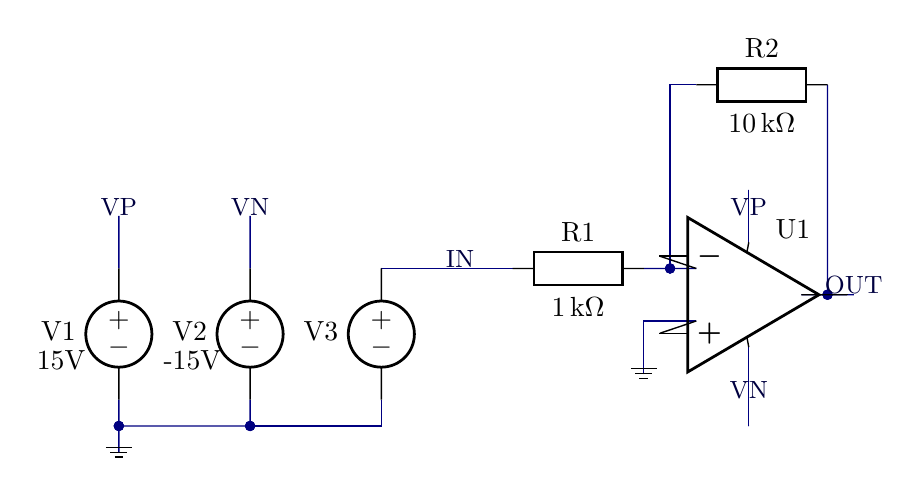
\begin{tikzpicture}[circuit ee IEC, scale=0.6666666667,line width=.5pt]% default: 0.4
	%\tikzstyle{every node}=[font=\small];%
	%\node [draw] at (0.0,0.0) {\pgfkeysvalueof{/tikz/circuitikz/tripoles/op amp/font}};
\draw [/lt2ti/Net](9.0,1.0)to[*short,-, color=netcolor] (9.0,1.0);% wire w3_w10 start
\draw [/lt2ti/Net](8.5,-2.5)to[*short,-*, color=netcolor] (8.5,-2.5);% wire w3_w10 end
\draw [/lt2ti/Net](9.0,1.0) --  (8.5,1.0) -- (8.5,-2.5); % wire w3_w10 polyline 
\draw [/lt2ti/Net](10.0,-2.0)to[*short,-, color=netcolor] (10.0,-2.0);% wire w4_w5 start
\draw [/lt2ti/Net](10.0,-1.0)to[*short,-, color=netcolor] (10.0,-1.0);% wire w4_w5 end
\draw [/lt2ti/Net](10.0,-2.0) --  (10.0,-1.5) -- (10.0,-1.0); % wire w4_w5 polyline 
\draw [/lt2ti/Net](-2.0,-2.5)to[*short,-, color=netcolor] (-2.0,-1.5);% wire w6
\draw [/lt2ti/Net](0.5,-2.5)to[*short,-, color=netcolor] (0.5,-1.5);% wire w7
\draw [/lt2ti/Net](5.5,-2.5)to[*short,-, color=netcolor] (5.5,-2.5);% wire w8_w9 start
\draw [/lt2ti/Net](3.0,-2.5)to[*short,-, color=netcolor] (3.0,-2.5);% wire w8_w9 end
\draw [/lt2ti/Net](5.5,-2.5) --  (4.5,-2.5) -- (3.0,-2.5); % wire w8_w9 polyline 
\draw [/lt2ti/Net](8.5,-2.5)to[*short,*-, color=netcolor] (8.0,-2.5);% wire w11
\draw [/lt2ti/Net](9.0,-2.5)to[*short,-*, color=netcolor] (8.5,-2.5);% wire w12
\draw [/lt2ti/Net](11.5,-3.0)to[*short,*-, color=netcolor] (11.5,1.0);% wire w13
\draw [/lt2ti/Net](11.5,-3.0)to[*short,*-, color=netcolor] (11.0,-3.0);% wire w14
\draw [/lt2ti/Net](12.0,-3.0)to[*short,-*, color=netcolor] (11.5,-3.0);% wire w15
\draw [/lt2ti/Net](9.0,-3.5)to[*short,-, color=netcolor] (9.0,-3.5);% wire w16_w17 start
\draw [/lt2ti/Net](8.0,-4.5)to[*short,-, color=netcolor] (8.0,-4.5);% wire w16_w17 end
\draw [/lt2ti/Net](9.0,-3.5) --  (8.0,-3.5) -- (8.0,-4.5); % wire w16_w17 polyline 
\draw [/lt2ti/Net](-2.0,-5.5)to[*short,*-, color=netcolor] (-2.0,-5.0);% wire w19
\draw [/lt2ti/Net](0.5,-5.5)to[*short,*-, color=netcolor] (0.5,-5.0);% wire w20
\draw [/lt2ti/Net](0.5,-5.5)to[*short,*-*, color=netcolor] (-2.0,-5.5);% wire w21
\draw [/lt2ti/Net](3.0,-5.0)to[*short,-, color=netcolor] (3.0,-5.0);% wire w22_w23 start
\draw [/lt2ti/Net](0.5,-5.5)to[*short,-*, color=netcolor] (0.5,-5.5);% wire w22_w23 end
\draw [/lt2ti/Net](3.0,-5.0) --  (3.0,-5.5) -- (0.5,-5.5); % wire w22_w23 polyline 
\draw [/lt2ti/Net](10.0,-5.5)to[*short,-, color=netcolor] (10.0,-5.5);% wire w18_w24 start
\draw [/lt2ti/Net](10.0,-4.0)to[*short,-, color=netcolor] (10.0,-4.0);% wire w18_w24 end
\draw [/lt2ti/Net](10.0,-5.5) --  (10.0,-5.0) -- (10.0,-4.0); % wire w18_w24 polyline 
\draw [/lt2ti/Net](-2.0,-6.0)to[*short,-*, color=netcolor] (-2.0,-5.5);% wire w25
 \draw (8.0, -4.5) node[ground, xscale=1, yscale=1, rotate=270, ] (undefined) {};%  (undefined)++(0.0,0.0) node {undefined }; % component "circuiTikz\gnd" "undefined" 
 \draw (-2.0, -6.0) node[ground, xscale=1, yscale=1, rotate=270, ] (undefined) {};%  (undefined)++(0.0,0.0) node {undefined }; % component "circuiTikz\gnd" "undefined" 
 \draw (10.08863, -3.0) node[op amp, xscale=1, rotate=0, ] (U1) {}  (U1)++(1*0.75,  1*1.25) node {U1 }; % component "OpAmps/ADA4817" "U1" 
 \draw (10.0,-2.0) to [*short, -] (U1.up);   \draw (10.0,-4.0) to [*short, -] (U1.down); % supply % component "OpAmps/ADA4817" "U1" 
 \draw (9.0,-3.5) to [*short, -] (U1.+);   \draw (9.0,-2.5) to [*short, -] (U1.-); \draw (11.0,-3.0) to [*short, -] (U1.out); % in/out % component "OpAmps/ADA4817" "U1" 
  \draw (-2.0, -2.5) to[*V, l_=V1, ,, -, ] (-2.0,-5.0){}; % component "voltage" "V1" 
  \draw (-3.1, -4.8) node[label=15V] {};
  \draw (0.5, -2.5) to[*V, l_=V2, ,, -, ] (0.5,-5.0){}; % component "voltage" "V2" 
  \draw (-0.6, -4.8) node[label=-15V] {};
  \draw (3.0, -2.5) to[*V, l_=V3, a^=,, -, ] (3.0,-5.0){}; % component "voltage" "V3" 
  \draw (8.0, -2.5) to[*resistor, a_=R1, l^=\SI{1}{\kilo\ohm}, -, ] (5.5,-2.5){}; %\node [] at (8.5,-2.0) {x}; % component "res" "R1" 
  \draw (11.5, 1.0) to[*resistor, a_=R2, l^=\SI{10}{\kilo\ohm}, -, ] (9.0,1.0){}; %\node [] at (12.0,1.5) {x}; % component "res" "R2" 
  \node (OUT) [] at (12.0,-3.0) {};% label mark % label "" "OUT" lbl28 
  \node (OUTtxt) [ netlabelcolor, above= -0.24cm of OUT] {{\pgfkeysvalueof{/lt2ti/netlabel/font}OUT}}; % label "" "OUT" lbl28 
  \node (VP) [] at (10.0,-1.5) {};% label mark % label "" "VP" lbl30 
  \node (VPtxt) [ netlabelcolor, above= -0.24cm of VP] {{\pgfkeysvalueof{/lt2ti/netlabel/font}VP}}; % label "" "VP" lbl30 
  \node (VP) [] at (-2.0,-1.5) {};% label mark % label "" "VP" lbl31 
  \node (VPtxt) [ netlabelcolor, above= -0.24cm of VP] {{\pgfkeysvalueof{/lt2ti/netlabel/font}VP}}; % label "" "VP" lbl31 
  \node (VN) [] at (0.5,-1.5) {};% label mark % label "" "VN" lbl32 
  \node (VNtxt) [ netlabelcolor, above= -0.24cm of VN] {{\pgfkeysvalueof{/lt2ti/netlabel/font}VN}}; % label "" "VN" lbl32 
  \node (VN) [] at (10.0,-5.0) {};% label mark % label "" "VN" lbl33 
  \node (VNtxt) [ netlabelcolor, above= -0.24cm of VN] {{\pgfkeysvalueof{/lt2ti/netlabel/font}VN}}; % label "" "VN" lbl33 
  \node (IN) [] at (4.5,-2.5) {};% label mark % label "" "IN" lbl34 
  \node (INtxt) [ netlabelcolor, above= -0.24cm of IN] {{\pgfkeysvalueof{/lt2ti/netlabel/font}IN}}; % label "" "IN" lbl34 

	\end{tikzpicture}
\end{document}
